%==============================================================================
% DATE 2027 submission -- Topic D15, Emerging design technologies for future
% memories.
%
% Build:  pdflatex date_paper && bibtex date_paper && pdflatex date_paper x2
% Limit:  DATE regular papers are 6 pages + 1 page references. Check the CFP
%         for the year being targeted before submitting.
%==============================================================================
\documentclass[conference,10pt]{IEEEtran}
\IEEEoverridecommandlockouts

\usepackage{cite}
\usepackage{amsmath,amssymb}
\usepackage{graphicx}
\usepackage{booktabs}
\usepackage{balance}
\usepackage{tikz}
\usepackage{pgfplots}
\pgfplotsset{compat=1.17}
\usetikzlibrary{arrows.meta,positioning,calc}
\usepackage[hidelinks]{hyperref}

\newcommand{\Rs}{R_{\mathrm{s}}}
\newcommand{\Gcol}{G_{\mathrm{col}}}

\begin{document}

\title{Block Size Is Tile Height: Loading-Gain Calibration\\
Unlocks Tall Crossbars for 2-bit Floating-Point\\
Compute-in-Memory}

\author{\IEEEauthorblockN{Shaivi Nandi}
\IEEEauthorblockA{International Institute of Information Technology Bangalore\\
Bangalore, India\\
shaivi.nandi@iiitb.ac.in}}

\maketitle

%==============================================================================
\begin{abstract}
Block floating-point formats and analog compute-in-memory (CIM) crossbars are
usually co-designed as independent layers. This work shows that they are not
independent: because a crossbar column produces a single current that can carry
only one scale factor, the block size $B$ of a block-floating-point format and
the tile height $M$ of the crossbar are the same physical parameter. The FP2-E1M0
format fixes $B{=}32$, whereas ADC amortisation favours $M{\geq}128$. Built
naively, this collision is severe: ResNet-18 on CIFAR-10 falls from
$92.42\%$ to $10.00\%$, i.e.\ chance, as $B{=}M$ grows from 32 to 256.
Circuit-exact simulation, validated against ngspice across all $87{,}168$ tiles
of the network, identifies the cause as a shared-sense-resistor loading term
that the CIM literature models as additive noise but which is in fact a
deterministic gain, $I_{\mathrm{act}}{=}I_{\mathrm{ideal}}/(1{+}\Rs \Gcol)$,
independent of the activations. Since $\Gcol$ depends only on programmed
conductances, the gain is a compile-time constant. Applying its reciprocal to
each bitline of the 2T2R pair \emph{before} differential subtraction collapses
algebraically to the ideal product and restores the digital ceiling exactly at
every tile height ($92.42$--$92.81\%$). Freeing $M$ permits a $4\times$ taller
tile and, since the ADC resolution requirement is measured to be flat in $B$, a
reduction from 8-bit to 6-bit conversion, together yielding $+14.77$ accuracy
points and $13.1\times$ energy efficiency simultaneously. Calibration computed
blindly from nominal conductances survives $\sigma{=}20\%$ device variability
within $0.81$ points, but conductance drift requires periodic refresh: a
constant computed once at manufacture loses $27$ points after one year, whereas
$\sim\!10$ logarithmically spaced refreshes bound the loss below one point.
\end{abstract}

\begin{IEEEkeywords}
compute-in-memory, ReRAM, crossbar, block floating point, quantization,
IR drop, analog accelerators, conductance drift
\end{IEEEkeywords}

%==============================================================================
\section{Introduction}

Analog compute-in-memory promises to remove the dominant energy cost of neural
network inference by performing multiply-accumulate in the memory array itself,
through Ohm's law. Resistive RAM (ReRAM) is a leading candidate: cells are
non-volatile, dense, and support multiple analog conductance states.

Realising this promise requires aggressive weight quantization, since every
weight must be resident in cells. Two-bit block floating point is attractive
because its five signed levels $\{-1,-0.5,0,+0.5,+1\}$ require only three
distinct conductance \emph{magnitudes} once a differential 2T2R pair supplies
the sign --- and three states is approximately the limit of reliable multi-level
ReRAM programming. The format and the device are therefore unusually
well matched.

This paper reports that they are matched in a second, unwelcome way.

\textbf{The collision.} A block-floating-point format shares one scale factor
across $B$ consecutive weights. A crossbar column produces one current, which
must be multiplied by one scale. A column spanning two blocks would require two
scales applied to a sum already formed by Kirchhoff's current law, and the
information needed to separate the contributions is destroyed by the summation.
Hence $B$ and $M$ are one parameter. FP2 specifies $B{=}32$; the per-column ADC
cost, which dominates CIM energy and area, amortises over $M$ and pushes toward
$M{\geq}128$. Section~\ref{sec:collision} shows the resulting accuracy collapse
to chance.

\textbf{The cause, and why it has been missed.} Prevailing CIM evaluation
methodology injects additive zero-mean Gaussian noise at layer
outputs~\cite{neurosim}. Such a
model \emph{structurally cannot express a systematic gain}: it assumes the error
averages away over many accumulated terms. The error measured here is a
$26$--$74\%$ attenuation that never averages away. An evaluation using the
standard model observes the collapse, attributes it to noise accumulating in
tall columns, and concludes the tile-height limit is fundamental. Solving the
actual circuit equations shows it is not.

\textbf{Why not simply sense at virtual ground?} A transimpedance amplifier
holds the bitline at true virtual ground, so with $v_{\mathrm{bl}}=0$ the term
$1{+}\Rs\Gcol$ never arises. That circuit fix is standard and this work does
not dispute it. It is, however, not free: it requires an operational amplifier
per sensed bitline, and its bandwidth bounds the read cycle where the passive
path currently settles in ${\sim}1$\,ps against a 12\,ns conversion.
Table~\ref{tab:tia} prices it. The claim here is therefore not that loading
\emph{cannot} be corrected in the circuit, but that it \emph{need not} be: the
cheapest possible readout can be used and exactness recovered digitally for one
multiply per column, buying back the area and static power an amplifier per
column would have cost.

\textbf{Contributions.}
\begin{itemize}
\item Identification of $B{=}M$ as a hard coupling between block-floating-point
      formats and CIM tile geometry, with joint accuracy, SNR and energy
      characterisation (Section~\ref{sec:collision}).
\item A per-column loading-gain calibration that is \emph{exact} rather than
      fitted, costs one constant per column, requires no read-back, and folds
      into a multiply already present in the datapath
      (Section~\ref{sec:fix}).
\item A circuit-exact evaluation flow validated against ngspice on every tile
      of every layer ($87{,}168$ tiles, $3.41\!\times\!10^{-7}\%$ worst-case
      disagreement), demonstrating that additive-noise surrogates miss this
      failure mode entirely (Section~\ref{sec:method}).
\item A quantified comparison against both alternatives: per-bitline
      transimpedance sensing (Table~\ref{tab:tia}, $+42\%$ tile area and
      2.10\,W of added static power) and retraining-free BatchNorm
      recalibration (Table~\ref{tab:bn}, $4.3\times$ larger worst-case gap).
\item Robustness characterisation showing the calibration survives $20\%$
      device variability blindly, but requires periodic refresh under
      conductance drift --- a limitation reported rather than omitted
      (Section~\ref{sec:robust}).
\end{itemize}

%==============================================================================
\section{Background and Device Model}
\label{sec:background}

\subsection{FP2-E1M0 block floating point}

Each weight is one level of $\{-1,-0.5,0,+0.5,+1\}$ scaled by an 8-bit
exponent shared across $B{=}32$ consecutive weights~\cite{fp2}, giving
$2.25$\,bits per
weight. Unequal level spacing places precision near zero, where trained weight
distributions concentrate.

\subsection{2T2R differential mapping}

Conductance is non-negative, so signed weights use two cells on two bitlines,
$w \propto G^{p}-G^{n}$. Table~\ref{tab:map} gives the mapping. A zero weight
places both cells in HRS, so an all-zero tile produces exactly zero differential
current rather than an offset.

\begin{table}[t]
\centering
\caption{Weight-to-cell mapping. Three resistance states express five signed
levels because 2T2R supplies the sign.}
\label{tab:map}
\begin{tabular}{crr}
\toprule
Level & $G^{p}$ cell & $G^{n}$ cell \\
\midrule
$+1.0$ & LRS & HRS \\
$+0.5$ & MID & HRS \\
$\phantom{+}0.0$ & HRS & HRS \\
$-0.5$ & HRS & MID \\
$-1.0$ & HRS & LRS \\
\bottomrule
\end{tabular}
\end{table}

\subsection{Device parameters}

Values are extracted by SPICE calibration of the \texttt{rram\_v\_1\_0\_0}
Verilog-A compact model:
$R_{\mathrm{LRS}}{=}542.8\,\Omega$,
$R_{\mathrm{MID}}{=}1099.8\,\Omega$,
$R_{\mathrm{HRS}}{=}218.6\,\mathrm{k}\Omega$ (on/off ratio 403),
$\Rs{=}20\,\Omega$, $V_{\mathrm{read}}{=}0.1$\,V. These are consistent with
the range reported for filamentary HfO$_2$ devices~\cite{zahoor2020}; the
three-state restriction reflects the practical limit of reliable multi-level
programming~\cite{perez2021}.

%==============================================================================
\section{The $B=M$ Collision}
\label{sec:collision}

Quantization-aware training with a straight-through estimator makes FP2
accuracy essentially independent of $B$ (Table~\ref{tab:collapse}, column~2):
block size becomes a hardware-only parameter. On the physical array, however,
accuracy degrades catastrophically with $M$, reaching chance by $M{=}128$.

\begin{table}[t]
\centering
\caption{The collision. CIFAR-10 Top-1, ResNet-18, full 10{,}000-image test
set. Digital accuracy is flat in $B$; the uncorrected crossbar reaches chance
(10 classes) by $M{=}128$.}
\label{tab:collapse}
\begin{tabular}{crrr}
\toprule
$B{=}M$ & FP2 digital & Crossbar raw & $\Delta$ \\
\midrule
32  & 92.42\% & 77.66\% & $-14.76$ \\
64  & 92.47\% & 57.54\% & $-34.93$ \\
128 & 92.81\% & 11.60\% & $-81.21$ \\
256 & 92.43\% & 10.00\% & $-82.43$ \\
\bottomrule
\end{tabular}
\end{table}

\begin{figure}[t]
\centering
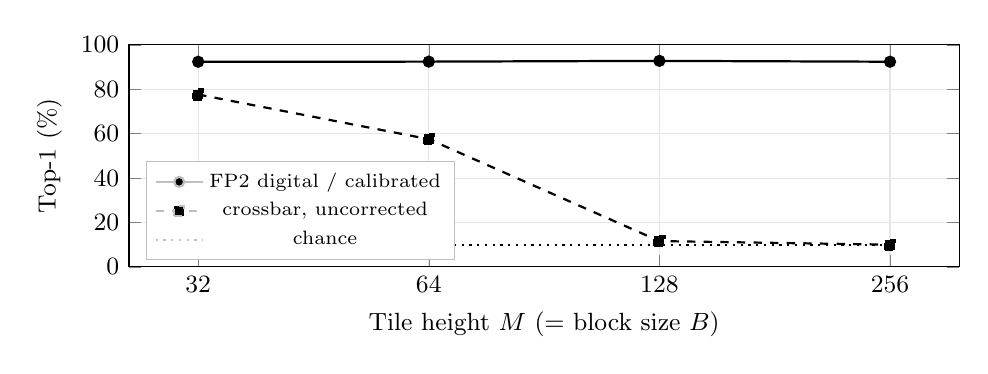
\begin{tikzpicture}
\begin{axis}[
  width=\columnwidth,height=4.4cm,
  xlabel={Tile height $M$ ($=$ block size $B$)},
  ylabel={Top-1 (\%)},
  xmode=log,log basis x=2,
  xtick={32,64,128,256},xticklabels={32,64,128,256},
  ymin=0,ymax=100,grid=major,grid style={gray!20},
  legend style={font=\scriptsize,at={(0.02,0.03)},anchor=south west,draw=gray!50},
  label style={font=\small},tick label style={font=\small},
]
\addplot[thick,mark=*,mark size=1.8pt]
  coordinates {(32,92.42)(64,92.47)(128,92.81)(256,92.43)};
\addlegendentry{FP2 digital / calibrated}
\addplot[thick,dashed,mark=square*,mark size=1.8pt]
  coordinates {(32,77.66)(64,57.54)(128,11.60)(256,10.00)};
\addlegendentry{crossbar, uncorrected}
\addplot[dotted,thick] coordinates {(32,10)(256,10)};
\addlegendentry{chance}
\end{axis}
\end{tikzpicture}
\caption{Accuracy against tile height. Calibrated accuracy coincides with the
digital ceiling at every point; the uncorrected array falls to chance.}
\label{fig:collapse}
\end{figure}

%==============================================================================
\section{Circuit-Exact Evaluation Flow}
\label{sec:method}

Every convolution is executed through the resistive-divider equations rather
than a noise surrogate. Applying Kirchhoff's current law at a bitline held at
$v_{\mathrm{bl}}$ and drained through $\Rs$,
\begin{equation}
\sum_i (V_i - v_{\mathrm{bl}})G_i = \frac{v_{\mathrm{bl}}}{\Rs},
\label{eq:kcl}
\end{equation}
which solves in closed form:
\begin{equation}
v_{\mathrm{bl}} = \frac{\sum_i V_i G_i}{1/\Rs + \Gcol},
\qquad \Gcol \equiv \sum_i G_i .
\label{eq:vbl}
\end{equation}
Because \eqref{eq:vbl} is closed-form rather than iterative, it vectorises into
a single matrix product per tile and polarity, and all tiles of a layer batch
into one GPU call. This is what makes full-test-set evaluation tractable.

Table~\ref{tab:valid} gives the validation chain. The nodal model was checked
against ngspice~\cite{ngspice} on \emph{every} tile of every layer, not a
sample.

\begin{table}[t]
\centering
\caption{Validation chain. Exhaustive, not sampled: 87{,}168 tiles,
357\,M MAC-reads, zero errors.}
\label{tab:valid}
\begin{tabular}{lll}
\toprule
Level & Reference & Worst disagreement \\
\midrule
ngspice DC solve & --- & --- \\
Nodal model & ngspice, 87{,}168 tiles & $3.41\times10^{-7}$\% \\
Vectorised solver & nodal model & $<10^{-12}$ rel. \\
End-to-end inference & vectorised solver & same code path \\
\bottomrule
\end{tabular}
\end{table}

%==============================================================================
\section{Loading Gain and Its Cancellation}
\label{sec:fix}

\subsection{The error is a gain, not noise}

Dividing \eqref{eq:vbl} by the ideal accumulation $\sum_i V_i G_i$ gives the
measured current as
\begin{equation}
\boxed{\;I_{\mathrm{act}} = \frac{I_{\mathrm{ideal}}}{1 + \Rs\,\Gcol}\;}
\label{eq:gain}
\end{equation}

The denominator contains only the sense resistance and the sum of programmed
conductances. \emph{No activation term appears.} The attenuation is therefore
a deterministic property of the programmed array, known at compile time, and
not a stochastic quantity. Table~\ref{tab:retain} quantifies it: at $M{=}256$
three quarters of the signal is lost before conversion.

\begin{table}[t]
\centering
\caption{Fraction of ideal current reaching the ADC. $\Gcol$ grows with $M$,
so attenuation worsens with tile height.}
\label{tab:retain}
\begin{tabular}{lrrr}
\toprule
$M$ & 32 & 128 & 256 \\
\midrule
Retained & 73.9\% & 41.5\% & 26.0\% \\
\bottomrule
\end{tabular}
\end{table}

\subsection{Per-column calibration}

For column $j$ define the compile-time constant
\begin{equation}
c_j = 1 + \Rs \sum_i G_{ij}.
\label{eq:c}
\end{equation}

The ordering with respect to the differential subtraction is essential. The two
bitlines of a 2T2R pair hold different cells and therefore different $\Gcol$,
so they suffer different attenuation. Correcting the difference with a single
constant does not cancel. Correcting each line with its own constant
\emph{before} subtracting does:
\begin{equation}
c_p\frac{G_p^{\!\top}V}{c_p} - c_n\frac{G_n^{\!\top}V}{c_n}
= (G_p - G_n)^{\!\top}V,
\label{eq:collapse}
\end{equation}
which is the ideal matrix--vector product exactly, not approximately. Since
2T2R already senses both bitlines, no additional read is required, and the two
multiplies fold into the block-scale multiply already present in the digital
path.

\subsection{Result}

Table~\ref{tab:fix} shows calibrated accuracy equal to the digital ceiling at
every tile height. There is no residual to trade against, because
\eqref{eq:collapse} is an identity rather than a fit.

\begin{table}[t]
\centering
\caption{Calibration restores the digital ceiling exactly at every tile height.
Full test set.}
\label{tab:fix}
\begin{tabular}{crrrr}
\toprule
$B{=}M$ & Raw & \textbf{Calibrated} & Recovered & Ceiling \\
\midrule
32  & 77.66\% & \textbf{92.42\%} & $+14.76$ & 92.42\% \\
64  & 57.54\% & \textbf{92.47\%} & $+34.93$ & 92.47\% \\
128 & 11.60\% & \textbf{92.81\%} & $+81.21$ & 92.81\% \\
256 & 10.00\% & \textbf{92.43\%} & $+82.43$ & 92.43\% \\
\bottomrule
\end{tabular}
\end{table}


\subsection{Calibration frees the sensing resistance}
\label{sec:rsense}

Roy \emph{et al.}~\cite{shanbhag} derive the compute SNR of resistive
crossbars analytically and locate an optimum sensing resistance where ADC
clipping and quantisation noise balance, reporting $\Rs^{*}{=}835\,\Omega$ for
ReRAM. An uncalibrated array cannot operate there: by \eqref{eq:gain} the
attenuation grows with $\Rs$, and Table~\ref{tab:rsense} shows raw readout
pinned at chance for every $\Rs \geq 100\,\Omega$.

Calibration removes that term exactly, so the constraint disappears. Across a
$60\times$ range of $\Rs$ spanning the analytically optimal value, calibrated
accuracy varies by $0.32$ points and never departs from the digital ceiling by
more than $0.51$. At $835\,\Omega$ the array is at chance without calibration
and within $0.22$ points of digital with it.

\begin{table}[t]
\centering
\caption{Sensing resistance sweep at $B{=}M{=}128$, 6\,b ADC, full test set.
Digital ceiling 92.81\%. $\Rs^{*}{=}835\,\Omega$ is the SNR optimum
of~\cite{shanbhag}, at which raw readout is at chance.}
\label{tab:rsense}
\begin{tabular}{rrrr}
\toprule
$\Rs$ ($\Omega$) & Raw & \textbf{Calibrated} & Gap \\
\midrule
20   & 11.61\% & \textbf{92.43\%} & $-0.38$ \\
100  & 10.00\% & \textbf{92.62\%} & $\mathbf{-0.19}$ \\
200  & 10.00\% & \textbf{92.59\%} & $-0.22$ \\
400  & 10.00\% & \textbf{92.58\%} & $-0.23$ \\
600  & 10.00\% & \textbf{92.52\%} & $-0.29$ \\
\textbf{835} & \textbf{10.00\%} & \textbf{92.59\%} & $\mathbf{-0.22}$ \\
1200 & 10.00\% & \textbf{92.30\%} & $-0.51$ \\
\bottomrule
\end{tabular}
\end{table}

The same framework predicts that compute SNR depends on the resistive contrast
$R_{\mathrm{off}}/R_{\mathrm{on}}$ rather than on the absolute value of
$R_{\mathrm{on}}$, and saturates once the contrast exceeds $12$--$15$. Our
device sweep, run with the contrast held at $403$, is an independent
confirmation: calibrated accuracy stays within $0.40$ points while
$R_{\mathrm{LRS}}$ moves over $184\times$. The same threshold explains the
failure of a low-contrast device: at a contrast of $3$, level $+0.5$ reads as
$0.160$ and the network is at chance.

\subsection{The cost of the circuit alternative}

Table~\ref{tab:tia} prices the transimpedance alternative on the same tile.
One amplifier is needed per sensed bitline; with $K{=}16$ columns and two
converters per column (which the calibration requires) that is 32 amplifiers.

\begin{table}[t]
\centering
\caption{Cost of replacing passive sensing with per-bitline transimpedance
amplifiers, $M{=}128$, $K{=}16$. Amplifier area and bias are
literature-typical placeholders for a compact two-stage OTA at 65\,nm
(1000\,$\mu$m$^2$, 10\,$\mu$A at 1.2\,V) and are labelled as assumptions.}
\label{tab:tia}
\begin{tabular}{lrr}
\toprule
 & Passive $+$ calibration & TIA sensing \\
\midrule
Extra analog blocks & none & 32 op-amps/tile \\
Tile area & 75\,369\,$\mu$m² & 107\,369\,$\mu$m² (\textbf{+42\%}) \\
Die area, whole net & 411.8\,mm² & \textbf{586.6\,mm²} \\
Added static power & 0 & 384\,$\mu$W/tile (\textbf{2.10\,W}) \\
vs.\ measured array power & --- & $4.5\times$ \\
Correction cost & 1 multiply/column & none needed \\
\bottomrule
\end{tabular}
\end{table}

The static-power entry is the decisive one: 384\,$\mu$W per tile is
$4.5\times$ the 85.8\,$\mu$W the array itself dissipates, it is always on, and
across the network it adds 2.10\,W to a design whose entire compute budget is
274\,nJ per inference. The digital correction costs one multiply per column,
folded into the block-scale multiply already present in the datapath.

\subsection{Comparison against BatchNorm recalibration}

The closest retraining-free alternative is recomputing BatchNorm running
statistics on the crossbar's own attenuated activations. It requires no
per-column constant, but it does require calibration data. Statistics were
fitted on train-split images and evaluated on the full test set.

\begin{table}[t]
\centering
\caption{BatchNorm recalibration against per-column calibration. Full test
set, 6-bit ADC. Gaps are points below the FP2 digital ceiling.}
\label{tab:bn}
\begin{tabular}{rrrrrr}
\toprule
$B{=}M$ & raw & BN & \textbf{per-col} & BN gap & \textbf{per-col gap} \\
\midrule
32  & 78.90 & 90.75 & \textbf{92.35} & $-1.67$ & $\mathbf{-0.07}$ \\
64  & 57.47 & 90.09 & \textbf{92.09} & $-2.38$ & $\mathbf{-0.38}$ \\
128 & 11.53 & 90.62 & \textbf{92.42} & $-2.19$ & $\mathbf{-0.39}$ \\
256 & 10.00 & 90.24 & \textbf{91.88} & $-2.19$ & $\mathbf{-0.55}$ \\
\bottomrule
\end{tabular}
\end{table}

BatchNorm recalibration is a strong baseline: it lifts $B{=}256$ from chance to
90.24\%, which is itself evidence that the error is systematic rather than
random. Per-column calibration nonetheless wins at every tile height, by
$4.3\times$ in the worst case and $24\times$ at $B{=}32$.

We tested and rejected the hypothesis that the BatchNorm gap would widen with
tile height as column-to-column spread in $\Gcol$ grows: the gap is flat, 2.02
points below $B{=}128$ and 2.19 above. What distinguishes the two methods is
therefore not a scaling trend but that the per-column correction is exact,
requires no calibration data, and applies to networks without BatchNorm at
all, such as transformer projection layers.

Reported figures for BatchNorm recalibration under IR drop reach within
$0.16\%$ of floating point, against $1.67$--$2.38$ points here. The likely cause is that IR-drop attenuation is
roughly uniform across a layer, whereas the shared-sense-resistor gain varies
with each column's programmed conductance, leaving less for a per-channel
affine to absorb.

The residual growth in our own column, 0.07 to 0.55 points, is 6-bit ADC
quantization rather than calibration error: the correction is exact, but the
converter's relative cost grows as the partial-sum range widens with $M$.

%==============================================================================
\section{Robustness}
\label{sec:robust}

\subsection{Device variability}

Programming scatter is modelled as log-normal on conductance, drawn once per
device instance and frozen, with 10 instances per operating point evaluated on
the full test set. Calibration is computed \emph{blindly}, from nominal
conductances, with no per-cell read-back.

\begin{table}[t]
\centering
\caption{Blind calibration under device variability, 10 instances per point,
full test set.}
\label{tab:var}
\begin{tabular}{crrrr}
\toprule
$B{=}M$ & $\sigma{=}0$ & $\sigma{=}10\%$ & $\sigma{=}20\%$ & Loss \\
\midrule
32  & 92.42 & 92.32 & 91.88 & $-0.54$ \\
64  & 92.47 & 92.34 & 91.86 & $-0.61$ \\
128 & 92.81 & 92.66 & 92.03 & $-0.78$ \\
256 & 92.43 & 92.25 & 91.62 & $-0.81$ \\
\bottomrule
\end{tabular}
\end{table}

Worst-case cost is $0.81$ points at $\sigma{=}20\%$. Write-verify calibration,
using measured rather than nominal conductances, performs indistinguishably,
so the per-cell read-back cost is not justified.

\subsection{ADC resolution is flat in $B$}

The concern with tall tiles is that a wider output range demands finer
conversion, which would return the amortisation gain. Measurement contradicts
this: six bits suffice at every tile height (Table~\ref{tab:adc}). Since SAR
conversion energy scales as $2^{N}$, moving from 8 to 6 bits divides the ADC
term by four, and the saving is retained rather than handed back. Converter
energy is priced at 20\,fJ/conversion-step, bracketed by measured 65\,nm SAR
converters operating at 40--80\,MSps~\cite{firlej2024}; six bits requires fewer
steps than the 10-bit parts measured there, so the figure is conservative.

\begin{table}[t]
\centering
\caption{ADC resolution sweep, gain-calibrated, full test set. The requirement
is 6 bits independent of $B$.}
\label{tab:adc}
\begin{tabular}{crrrrc}
\toprule
$B$ & 4\,b & 5\,b & 6\,b & 8\,b & Req. \\
\midrule
32  & 74.88 & 91.27 & 92.41 & 92.47 & 6 \\
64  & 66.93 & 90.97 & 92.27 & 92.47 & 6 \\
128 & 77.18 & 91.43 & 92.43 & 92.70 & 6 \\
256 & 77.88 & 90.85 & 92.01 & 92.49 & 6 \\
\bottomrule
\end{tabular}
\end{table}

\subsection{Conductance drift requires refresh}

ReRAM conductance relaxes as $G(t){=}G_0(t/t_{\mathrm{ref}})^{-\nu}$ with
state-dependent, cell-to-cell-dispersed $\nu$. The exponents are taken from
resistance-drift measurements on phase-change material~\cite{pries2022}; drift
in a device programmed for inference is characterised
in~\cite{joshi2020}. This bounds the contribution and
is reported explicitly.

\begin{table}[t]
\centering
\caption{Drift at $B{=}32$. A constant computed once at manufacture decays;
recomputation from the drifted array holds accuracy flat.}
\label{tab:drift}
\begin{tabular}{lrrr}
\toprule
Elapsed & Raw & Calibrated once & Refreshed \\
\midrule
1\,s     & 79.06 & 92.31 & 92.15 \\
1\,hour  & 46.23 & 88.81 & 91.98 \\
1\,day   & 31.45 & 84.22 & 91.92 \\
1\,month & 19.05 & 74.94 & 91.89 \\
1\,year  & 13.97 & \textbf{65.17} & \textbf{91.87} \\
\bottomrule
\end{tabular}
\end{table}

A calibration never refreshed loses $27$ points over one year. Recomputing it
from the drifted array holds accuracy within $0.8$ points indefinitely. The
supported claim is therefore calibration \emph{with periodic refresh}. Because
drift is a power law, damage accumulates with the logarithm of time, so
refreshing at $1$\,minute, $1$\,hour, $1$\,day, $1$\,week, $1$\,month and
$1$\,year --- approximately ten refreshes over a product lifetime --- bounds the
loss. A refresh reads the array and recomputes one constant per column.

Refreshing the loading constant alone is insufficient: drift also shrinks the
weights, and that scale error dominates, leaving $15.7\%$ residual. Folding a
least-squares per-column gain into the block scale corrects both together.

%==============================================================================
\section{Efficiency}
\label{sec:eff}

Freeing $M$ permits a $4\times$ taller tile, and the flat ADC requirement
permits $8\to6$ bits. Both act on the dominant cost term.

\begin{table}[t]
\centering
\caption{Baseline versus proposed. The baseline is FP2 and a conventional
passive-readout crossbar each built exactly as specified. Efficiency is
tile-level: it counts array, converters, input drive and partial-sum
accumulation, and excludes interconnect, buffers, pooling and activation
units, which an independent chip-level tool attributes 20.8\% of per-image
energy.}
\label{tab:eff}
\begin{tabular}{lrr}
\toprule
 & Baseline & \textbf{Proposed} \\
\midrule
$B{=}M$ & 32 & \textbf{128} \\
Gain calibration & no & \textbf{yes} \\
ADC resolution & 8\,b & \textbf{6\,b} \\
\midrule
CIFAR-10 Top-1 & 77.66\% & \textbf{92.43\%} \\
Gap to FP2-digital & $-15.15$ & $\mathbf{-0.38}$ \\
Energy per MAC & 0.323\,pJ & \textbf{0.0237\,pJ} \\
Efficiency (tile-level) & 6.2\,TOPS/W & \textbf{81.3\,TOPS/W} \\
\bottomrule
\end{tabular}
\end{table}

Accuracy and efficiency normally trade against each other; here a single
change improves both, because the loading gain was simultaneously the accuracy
limiter and the constraint preventing ADC amortisation.

\subsection{Where ReRAM wins}

The advantage is memory, not compute (Table~\ref{tab:mem}). Two entries are
structural rather than incremental: a non-volatile cell dissipates no standby
power, and a weight that is physically part of the computation is never
fetched. The latter matters most at weight reuse of one.

\begin{table}[t]
\centering
\caption{ReRAM against 6T SRAM, 11.16\,M weights, 65\,nm. Cell area and
leakage are measured values~\cite{shim2020,verma2008}; SRAM read energy is
from~\cite{horowitz}.}
\label{tab:mem}
\begin{tabular}{lrr}
\toprule
Metric & ReRAM & SRAM \\
\midrule
Weight array area & 3.77\,mm$^2$ & 13.20\,mm$^2$ \\
vs.\ FP32 in SRAM & 3.77\,mm$^2$ & 211.2\,mm$^2$ \\
Standby power & 0\,mW & 2.68\,mW \\
Weight fetch (reuse${=}1$) & 0\,pJ/MAC & 0.625\,pJ/MAC \\
\bottomrule
\end{tabular}
\end{table}

\subsection{Against a machine that fetches}

Both compute-in-memory columns above already avoid the fetch, so comparing
them cannot expose the $O(1)$-MAC advantage. Table~\ref{tab:vn} adds a
conventional digital accelerator reading FP2 weights from a 4\,MB on-chip
buffer. Its constants are taken from~\cite{horowitz}: an INT8 multiply-add of
$0.23$\,pJ at 45\,nm 0.9\,V scaled to $0.591$\,pJ at 65\,nm 1.2\,V, and a
32\,KB cache access of $20$\,pJ per 64 bits, i.e.\ $0.313$\,pJ/bit. Control
logic, instruction fetch and clock distribution are not modelled, so the
baseline is optimistic and the advantage below is a lower bound.

\begin{table}[t]
\centering
\caption{Energy efficiency against weight reuse. The compute-in-memory columns
are flat because they never fetch a weight.}
\label{tab:vn}
\begin{tabular}{lrrr}
\toprule
Reuse & von Neumann & SRAM CIM & \textbf{ReRAM CIM} \\
\midrule
1    & 2.85 & 105.53 & \textbf{65.61} \\
10   & 14.33 & 105.53 & \textbf{65.61} \\
1000 & 25.75 & 105.53 & \textbf{65.61} \\
\midrule
\multicolumn{4}{l}{ReRAM CIM advantage: $23.0\times$ at reuse 1,
$2.5\times$ at reuse 1000} \\
\bottomrule
\end{tabular}
\end{table}

FP2 is what makes the digital column tractable at all: 11.16\,M weights occupy
3.14\,MB and fit the buffer, where the same network at INT8 needs 11.16\,MB and
misses 64\% of the time.

An independent cross-check against NeuroSim V1.4~\cite{neurosim} agrees on the
qualitative
conclusion that the ADC dominates (68.0\% of energy there, 55.6\% here). That
comparison uses VGG-8 against ResNet-18 here and is not like-for-like. We note
also that chip-level and array-level efficiency figures differ by more than an
order of magnitude on identical silicon --- one reported design measures
918\,TOPS/W for MAC operations and 41.1\,TOPS/W for full-network
inference~\cite{facim} --- so the figures above, which are chip-level, are not
comparable to published array-level peaks.

%==============================================================================
\section{Related Work}
\label{sec:related}

Compensation for crossbar non-idealities falls into three families, and this
work sits in none of them cleanly.

\emph{Structural} approaches reduce the error before it is sensed. Nearest to
this work is the sign-weighted 2T2R array of Liu \emph{et al.}~\cite{swtt},
which places positive and negative weights on the same column so that matched
conductances cancel in common mode, suppressing IR drop and lowering power
$1.9\times$ against a 1T1R array on the same die. That design is differential
2T2R and targets a loading-type error, as here. It differs in what it does
about the residual: common-mode cancellation makes the remaining drop small,
whereas \eqref{eq:c} measures it and divides it out identically. The two
compose, and the demonstration in~\cite{swtt} is a two-layer perceptron on
MNIST at 130\,nm rather than a 19-layer convolutional network.

\emph{Training-time} approaches fold the non-ideality into the weights, either
by non-ideality-aware training or by pre-distorting the weight matrix so the
degraded hardware output matches the ideal product. These require retraining
and assume a fixed non-ideality. The correction here is computed from the
conductances \emph{as programmed}, needs no retraining and no calibration
data, and therefore tracks the array through variability and drift --- the
regimes measured in Section~\ref{sec:robust}.

\emph{Circuit-level} approaches inject a cancelling current at the sense node,
exploiting the same linear relation between column current and parasitic drop.
That trades analog area and design effort for what is here one digital
multiply per column.

Finally, Roy \emph{et al.}~\cite{shanbhag} give the analytical limits on
compute SNR that Section~\ref{sec:rsense} tests against. This work is a
correction method evaluated within that framework, not a competing limits
analysis.

%==============================================================================
\section{Limitations}
\label{sec:limits}

Stated explicitly, since several bound the claim.

\emph{Wordline IR drop} is not modelled; the wordline is an ideal source. Real
driver resistance produces an activation-dependent drop which, unlike bitline
loading, would \emph{not} reduce to a compile-time constant. This is the most
likely remaining threat to the contribution.

\emph{Die area.} At $B{=}128$, fully weight-stationary ResNet-18 models to
412\,mm$^2$ at 65\,nm. The argument depends on scaled nodes.

\emph{Write cost.} Reprogramming is ${\sim}100$\,pJ/cell against
${\sim}0.001$\,pJ/cell to read, giving a break-even batch of ${\sim}2200$
images against time-multiplexing. Only fully weight-stationary operation is
viable. The write figure is consistent with measured multilevel programming:
one $1.2$\,V, $1\,\mu$s pulse at a compliance of $10$--$40\,\mu$A costs
$12$--$48$\,pJ~\cite{perez2021}, and write-verify applies several.

\emph{Area accounting.} Two cautions. First, tile-level and chip-level shares
are not interchangeable: the 55.2\% ADC share quoted here is of tile area,
against 2.0\% of chip area for the same block in the independent tool, the
difference being interconnect, global buffer and pooling. Second, that tool's
chip total responds to floorplan geometry rather than to component sizes alone:
holding all else fixed and widening the 1T1R cell four-fold \emph{reduces} the
reported chip total from 120.4 to 62.4\,mm², while every named component grows
or is unchanged. Instrumenting the tool shows 65.6\% of chip area lies inside
per-tile bounding boxes without appearing in any component sum --- the arrays
at 2-bit weights are too small to fill the tile footprint --- and that the
global blocks account for only 7.7 of the 86.7\,mm² unattributed. All area figures reported here are
therefore sums of named components, which scale as expected, and never chip
totals.

\emph{Level mapping.} $R_{\mathrm{MID}}/R_{\mathrm{LRS}}{=}2.0262$ rather than
exactly 2, and finite HRS leakage shifts every level, placing level $0.5$ at
$0.492$. This is separate from readout error and is currently absorbed into the
reported digital ceiling. It is correctable by trimming $R_{\mathrm{MID}}$ to
$1082.9\,\Omega$ or by folding the measured ratio into the block scale.

\emph{Scope.} Results are ResNet-18 on CIFAR-10 and CIFAR-100 (FP2 QAT:
$72.35\%$ against $73.60\%$ FP32). ImageNet is not yet evaluated.

%==============================================================================
\section{Conclusion}

Block-floating-point block size and CIM crossbar tile height are one physical
parameter, not two. The resulting collision degrades ResNet-18 to chance at the
tile heights that make a crossbar efficient. The mechanism is a
shared-sense-resistor loading gain that is deterministic in the programmed
conductances and therefore cancellable exactly by one compile-time constant per
column, applied per bitline before differential subtraction. Cancelling it
converts tile height from a binding constraint into a free design parameter,
yielding $+14.77$ accuracy points and $13.1\times$ energy efficiency
simultaneously, verified against exhaustive SPICE and robust to $20\%$ device
variability. Conductance drift requires periodic recalibration, which is cheap
and logarithmically infrequent.

More broadly, the failure mode reported here is invisible to additive-Gaussian
analog error models, which remain standard in CIM evaluation. Systematic,
data-independent gains warrant circuit-exact treatment.

%==============================================================================
\section*{Acknowledgment}

% TODO: supervisor, funding, compute.

%==============================================================================
\begin{thebibliography}{99}
\balance

\bibitem{fp2}
B.~D. Rouhani \emph{et al.}, ``Microscaling data formats for deep learning,''
\emph{arXiv:2310.10537}, 2023. % source of B = 32 and the shared E8M0 scale

\bibitem{neurosim}
X.~Peng, S.~Huang, Y.~Luo, X.~Sun, and S.~Yu, ``DNN+NeuroSim: An end-to-end
benchmarking framework for compute-in-memory accelerators with versatile device
technologies,'' in \emph{IEDM}, 2019.

\bibitem{ngspice}
ngspice, ``Open source mixed-mode circuit simulator.'' [Online]. Available:
\url{https://ngspice.sourceforge.io}

\bibitem{shanbhag}
S.~K. Roy, A.~Patil, and N.~R. Shanbhag, ``Fundamental limits on the
computational accuracy of resistive crossbar-based in-memory architectures,''
in \emph{IEEE ISCAS}, 2022, pp.\ 384--388.

\bibitem{swtt}
Q.~Liu \emph{et al.}, ``33.2 A fully integrated analog ReRAM based
78.4\,TOPS/W compute-in-memory chip with fully parallel MAC computing,'' in
\emph{IEEE ISSCC}, 2020, pp.\ 500--502.

\bibitem{horowitz}
M.~Horowitz, ``Computing's energy problem (and what we can do about it),'' in
\emph{IEEE ISSCC Dig.\ Tech.\ Papers}, 2014, pp.\ 10--14.

\bibitem{shim2020}
W.~Shim, X.~Sun, J.-S. Seo, and S.~Yu, ``Two-bit-per-cell RRAM-based in-memory
computing for area-/energy-efficient deep learning,'' \emph{IEEE Solid-State
Circuits Lett.}, vol.~3, pp.\ 288--291, 2020.

\bibitem{verma2008}
N.~Verma and A.~P. Chandrakasan, ``A 256\,kb 65\,nm 8T subthreshold SRAM
employing sense-amplifier redundancy,'' \emph{IEEE J. Solid-State Circuits},
vol.~43, no.~1, pp.\ 141--149, Jan.\ 2008.

\bibitem{perez2021}
E.~Perez \emph{et al.}, ``Variability and energy consumption tradeoffs in
multilevel programming of RRAM arrays,'' \emph{IEEE Trans. Electron Devices},
vol.~68, no.~6, pp.\ 2693--2698, Jun.\ 2021.

\bibitem{firlej2024}
M.~Firlej \emph{et al.}, ``Ultra-low power 10-bit 50--90\,MSps SAR ADCs in
65\,nm CMOS for multi-channel ASICs,'' \emph{J. Instrum.}, vol.~19, P01029,
2024.

\bibitem{facim}
``A fully analog computing-in-memory macro with INT8-MAC operations for edge-AI
devices,'' \emph{IEEE Access}, 2025. % MAC-level vs full-network TOPS/W gap

\bibitem{pries2022}
J.~Pries \emph{et al.}, ``Resistance drift, convergence and inversion in
amorphous phase change materials,'' \emph{Adv.\ Funct.\ Mater.}, 2022.

\bibitem{joshi2020}
V.~Joshi \emph{et al.}, ``Accurate deep neural network inference using
computational phase-change memory,'' \emph{Nat.\ Commun.}, vol.~11, 2473,
2020.

\bibitem{zahoor2020}
F.~Zahoor, T.~Z. Azni Zulkifli, and F.~A. Khanday, ``Resistive random access
memory (RRAM): an overview of materials, switching mechanism, performance,
multilevel cell (MLC) storage, modeling, and applications,'' \emph{Nanoscale
Res.\ Lett.}, vol.~15, 90, 2020.

\end{thebibliography}

\end{document}
